\chapter{Visual recognition}
The pictures accompanying the posts usually help a lot in determining the emotion of the user. For instance, happy photos might contain landscapes with the sun or a beach while sad ones might have really dark colors. To analyse the images, we'll use convolutional neural networks, which achieve state-of-the-art performances in many visual recognition tasks. First we'll explain how they work and then we'll dive into the architecture we've used for deep sentiment analysis.
%%%%%%%%%%%%%%%%%%%%%%%%%%%%%%%%%%%%%%%%%%%%%%%%%%%%%%%%%%%%
%%%%%%%%%%%%%%%%%%%%  NEW SECTION   %%%%%%%%%%%%%%%%%%%%%%%%
%%%%%%%%%%%%%%%%%%%%%%%%%%%%%%%%%%%%%%%%%%%%%%%%%%%%%%%%%%%%
\section{Convolutional neural networks}
A convolutional neural networks, often called ConvNets, can be seen as a simulation of the human visual cortex, that is to say an aggregation of plenty of receptive fields. (some illustrations might be helpful here)

\subsection{Convolutional layer}
Take an image of dimension $(h,w,3)$ with $h$ the height, $w$ the width and 3 representing the number of channels (red, blue, green). If you simply flatten that image and transform it into a vector of size $h\times h \times 3$ and feed that vector to a neural network, you'll get not-so-good results as you've thrown away all the spatial information. Convolutions extract that spatial information and work the following way:
\begin{itemize}
\item Each convolution is described by a filter F of size $(f, f, 3)$, $f$ usually being in the range $[1,13]$.
\item Position the filter on the upper left of the image and element-wise multiply with the filter, then sum those numbers to obtain a raw number.
\item Slide across the image, one pixel at a time horizontally and vertically, and repeat the previous operation.
\end{itemize}

\begin{figure}
\begin{subfigure}[t]{.5\textwidth}
  \vskip 0pt
  \centering
  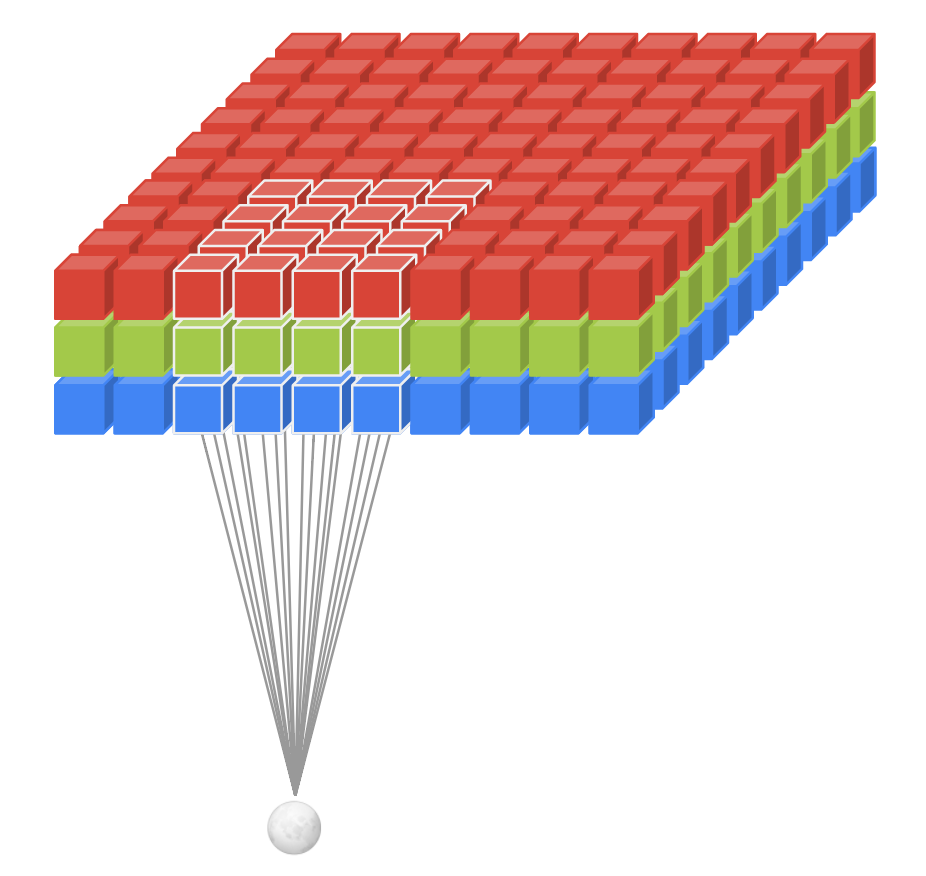
\includegraphics[width=.8\linewidth]{Images/conv1.png}
  \caption{One operation of convolution}
\end{subfigure}
\begin{subfigure}[t]{.5\textwidth}
  \vskip 0pt 
  \centering
  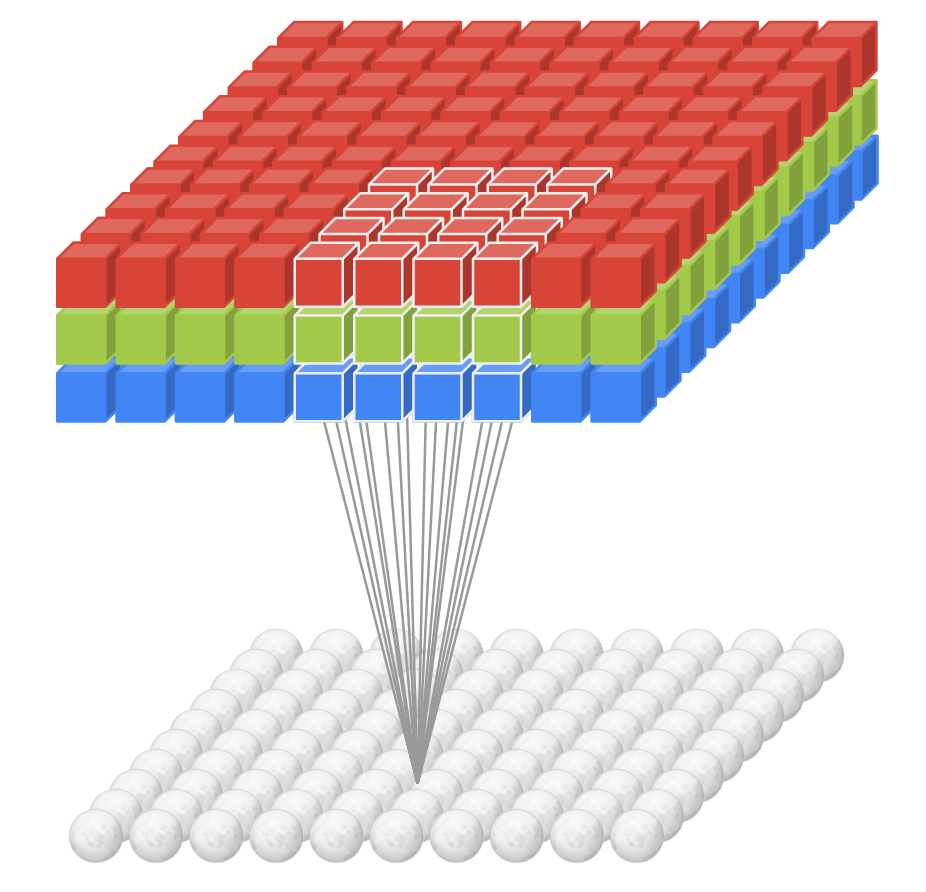
\includegraphics[width=.8\linewidth]{Images/conv2.png}
  \caption{The result of the convolution}
\end{subfigure}
\caption{A convolution, each neuron been a `receptive field' \cite{gorner}}
\end{figure}

By sliding through the image, you would get a new matrix of dimension $(h_{new}, w_{new},1)$, with $h_{new}=h-f+1$ and $w_{new}=w-f+1$. However, we usually don't want to reduce the size of our input image that fast, as we usually have several convolutions. To ensure that the image has the same size, zero-padding is used: we add $p$ zeros to the borders of the input image to preserve the spatial size of the input. With zero-padding, $h_{new}$ becomes: $h_{new} =  h + 2p - f + 1$, and we want that $h_{new}$ equals $h$:
$$ h + 2p - f + 1 = h$$
Therefore, $p=\frac{f-1}{2}$.

A convolution extract information about the image such as edges or blotches of some color (Figure \ref{conv-ex}). The grayscale and edges filters were hardcoded but in a ConvNet setting, the weights of the filter F are learned through optimising a loss function -- in our case, a metric measuring how accurate our predictions of the emotions are. The network will learn weights that will detect features that will be most relevant to our specific task. Most of the time, more than a single convolution are used: just repeat that operation $d$ (the depth) times, to create a new tensor of dimension $(h,w,d)$. We can then apply convolutions on that new image. First layers will recognise simple features such as edges or aggregation of colors, and deeper layers might activate on faces, wheels and so on.

\begin{figure}
\centering
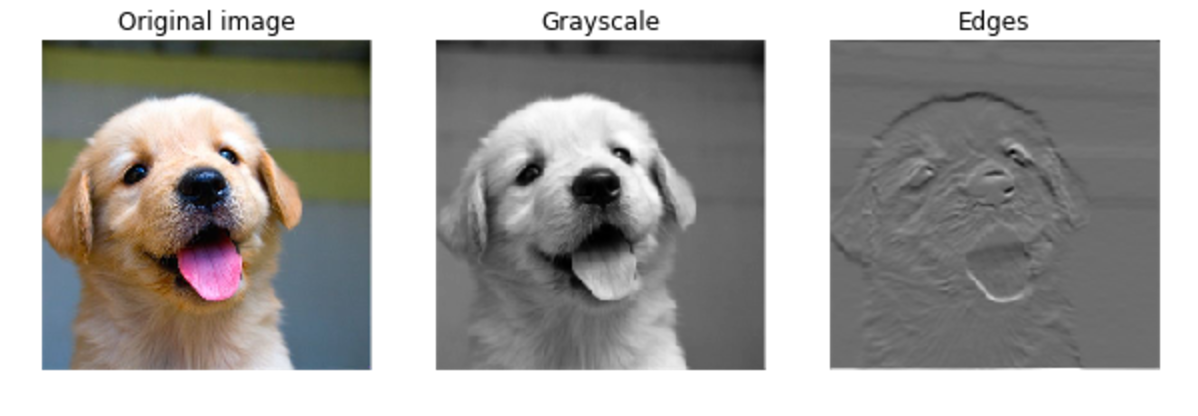
\includegraphics[width=0.8\textwidth]{Images/conv_ex.png}
\caption{Examples of convolution}
\label{conv-ex}
\end{figure}

\subsection{Pooling layer}
After a few iterations of convolutions, inserting pooling layers in-between convolutional layers might be a good idea to control the spatial complexity of the network. More concretely, what is most used in practice is the 2x2 max-pooling:
\begin{itemize}
\item Pick a channel among the $d$ ones.
\item Position yourself on the top-left 2x2 square of the image and take the max.
\item Repeat by sliding through the image vertically and horizontally with a stride (step) of 2.
\end{itemize}

\begin{figure}
\centering
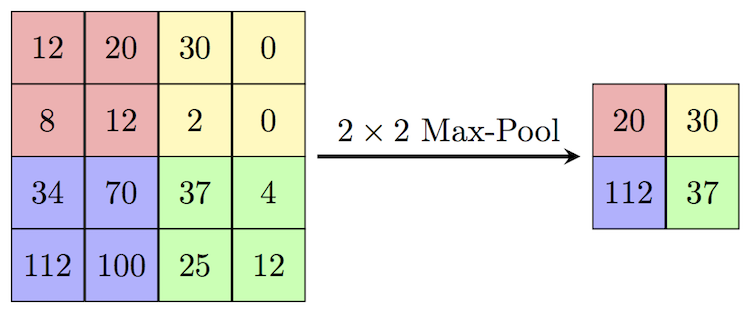
\includegraphics[width=0.8\textwidth]{Images/maxpool.png}
\caption{Max pooling \cite{camb-spark}}
\end{figure}

After applying max pooling to each channel, the resulting image's dimension is $(\frac{h}{2}, \frac{w}{2}, d)$ and we have discarded 75\% of the neurons (as in each max-pool operation, we only keep the maximum neuron among the fours), effectively reducing the number of parameters and controlling overfitting.




